\let\negmedspace\undefined
\let\negthickspace\undefined
\documentclass[journal,12pt,onecolumn]{IEEEtran}
\usepackage{cite}
\usepackage{amsmath,amssymb,amsfonts,amsthm}
\usepackage{algorithmic}
\usepackage{graphicx}
\graphicspath{{./figs/}}
\usepackage{textcomp}
\usepackage{xcolor}
\usepackage{txfonts}
\usepackage{listings}
\usepackage{enumitem}
\usepackage{mathtools}
\usepackage{gensymb}
\usepackage{comment}
\usepackage{caption}
\usepackage[breaklinks=true]{hyperref}
\usepackage{tkz-euclide} 
\usepackage{listings}
\usepackage{gvv}                                        
%\def\inputGnumericTable{}                                 
\usepackage[latin1]{inputenc}     
\usepackage{xparse}
\usepackage{color}                                            
\usepackage{array}                                            
\usepackage{longtable}                                       
\usepackage{calc}                                             
\usepackage{multirow}
\usepackage{multicol}
\usepackage{hhline}                                           
\usepackage{ifthen}                                           
\usepackage{lscape}
\usepackage{tabularx}
\usepackage{array}
\usepackage{float}
\newtheorem{theorem}{Theorem}[section]
\newtheorem{problem}{Problem}
\newtheorem{proposition}{Proposition}[section]
\newtheorem{lemma}{Lemma}[section]
\newtheorem{corollary}[theorem]{Corollary}
\newtheorem{example}{Example}[section]
\newtheorem{definition}[problem]{Definition}
\newcommand{\BEQA}{\begin{eqnarray}}
\newcommand{\EEQA}{\end{eqnarray}}
\newcommand{\define}{\stackrel{\triangle}{=}}
\theoremstyle{remark}
\newtheorem{rem}{Remark}

\begin{document}
\title{
ASSIGNMENT 5: GATE 2012 \\
    PH : PHYSICS }
\author{AI25BTECH11035 - Sujal Rajani }
\maketitle
\renewcommand{\thefigure}{\theenumi}
\renewcommand{\thetable}{\theenumi}
\section*{\textbf{General Aptitude (GA)}}
\textbf{Q.1 -- Q.5 Carry ONE mark Each} 
\begin{enumerate}
\item If $\rightarrow$ denotes increasing order of intensity, then the meaning of the words
[smile $\rightarrow$ giggle $\rightarrow$ laugh] is analogous to [disapprove $\rightarrow$ \underline{\hspace*{2em}} $\rightarrow$ chide].
Which one of the given options is appropriate to fill the blank?
\begin{enumerate}
    \item reprove
    \item praise
    \item reprise
    \item grieve
\end{enumerate}


\item Find the odd one out in the set: \{19, 37, 21, 17, 23, 29, 31, 11\}
\begin{enumerate}
    \item 21
    \item 29
    \item 37
    \item 23
\end{enumerate}

\item In the following series, identify the number that needs to be changed to form the Fibonacci series.
\hspace*{2em}1, 1, 2, 3, 6, 8, 13, 21, \ldots
\begin{enumerate}
    \item 8
    \item 21
    \item 6
    \item 13
\end{enumerate}


\item The real variables $x$, $y$, $z$, and the real constants $p$, $q$, $r$ satisfy\\
\begin{align*}
    \frac{x}{pq - r^2} = \frac{y}{qr - p^2} = \frac{z}{rp - q^2}
\end{align*}

Given that the denominators are non-zero, the value of $px + qy + rz$ is
\begin{enumerate}
    \item 0
    \item 1
    \item $pqr$
    \item $pqr$
\end{enumerate}

\item Take two long dice (rectangular parallelepiped), each having four rectangular faces labelled as 2, 3, 5, and 7. If thrown, the long dice cannot land on the square faces and has 1/4 probability of landing on any of the four rectangular faces. The label on the top face of the dice is the score of the throw.
If thrown together, what is the probability of getting the sum of the two long dice scores greater than 11?
\begin{enumerate}
    \item 3/8
    \item 1/8
    \item 1/16
    \item 3/16
\end{enumerate}

\item In the given text, the blanks are numbered (i)--(iv). Select the best match for all the blanks.\\
Prof. P \underline{(i)} merely a man who narrated funny stories. \underline{(ii)} in his blackest moments he was capable of self-deprecating humor.\\
Prof. Q \underline{(iii)} a man who hardly narrated funny stories. \underline{(iv)} in his blackest moments was he able to find humor.
\begin{enumerate}
    \item (i) was \hspace{1em} (ii) Only \hspace{1em} (iii) was not \hspace{1em} (iv) Even
    \item (i) was not \hspace{1em} (ii) Even \hspace{1em} (iii) was \hspace{1em} (iv) Only
    \item (i) was \hspace{1em} (ii) Even \hspace{1em} (iii) was not \hspace{1em} (iv) Only
    \item (i) was not \hspace{1em} (ii) Only \hspace{1em} (iii) was \hspace{1em} (iv) Even
\end{enumerate}


\item How many combinations of non-null sets A, B, C are possible from the subsets of $\{2,3,5\}$ satisfying the conditions: (i) A is a subset of B, and (ii) B is a subset of C?
\begin{enumerate}
    \item 28
    \item 27
    \item 18
    \item 19
\end{enumerate}

\item The bar chart gives the batting averages of VK and RS for 11 calendar years from 2012 to 2022. Considering that 2015 and 2019 are world cup years, which one of the following options is true?
\begin{figure}[H]
    \centering
    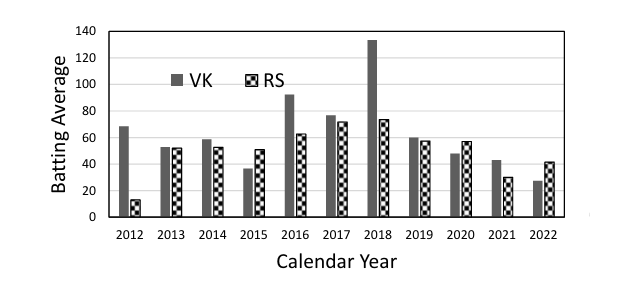
\includegraphics[width = 1\columnwidth]{fig/Q8.png}
    \caption*{}
    \label{fig:Q8}
\end{figure}
\begin{enumerate}
    \item RS has a higher yearly batting average than that of VK in every world cup year.
    \item VK has a higher yearly batting average than that of RS in every world cup year.
    \item VK yearly batting average is consistently higher than that of RS between the two world cup years.
    \item RS yearly batting average is consistently higher than that of VK in the last three years.
\end{enumerate}

\item A planar rectangular paper has two V-shaped pieces attached as shown below.
\begin{figure}[H]
    \centering
    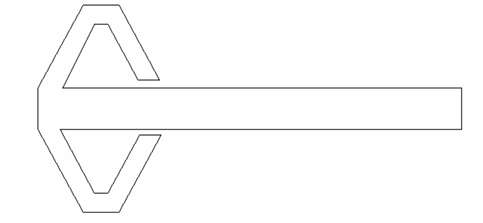
\includegraphics[width = 0.6\columnwidth]{fig/Q9.png}
    \caption*{}
    \label{fig:Q9}
\end{figure}
This piece of paper is folded to make the following closed three-dimensional object.
\begin{figure}[H]
    \centering
    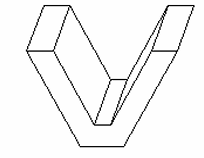
\includegraphics[width = 0.2\columnwidth]{fig/Q9(2).png}
    \caption*{}
    \label{fig:Q9(2)}
\end{figure}
The number of folds required to form the above object is
\begin{enumerate}
    \item 9
    \item 7
    \item 11
    \item 8
\end{enumerate}

\item Four equilateral triangles are used to form a regular closed three-dimensional object by joining along the edges. The angle between any two faces is
\begin{enumerate}
    \item 30$^\circ$
    \item 60$^\circ$
    \item 45$^\circ$
    \item 90$^\circ$
\end{enumerate}
\textbf{Q11-Q35 Carry ONE mark Each}
\item If $F_1(Q, q) = Qq$ is the generating function of a canonical transformation from $(p, q)$ to $(P, Q)$, then which one of the following relations is correct?
\begin{enumerate}
    \item $ \dfrac{p}{P} = \dfrac{Q}{q}$
    \item $ \dfrac{P}{p} = -\dfrac{Q}{q}$
    \item $\dfrac{p}{P} = -\dfrac{Q}{q}$
    \item $\dfrac{P}{p} = -\dfrac{Q}{q}$
\end{enumerate}


\item An unpolarized plane electromagnetic wave in a dielectric medium 1 is incident on a plane interface that separates medium 1 from another dielectric medium 2. Medium 1 and medium 2 have refractive indices $n_1$ and $n_2$, respectively, with $n_2 > n_1$. If the angle of incidence is $\tan^{-1}\brak{\frac{n_2}{n_1}} $, which one of the following statements is true?
\begin{enumerate}
    \item The reflected wave is unpolarized
    \item The reflected wave is polarized parallel to the plane of incidence
    \item The reflected wave is polarized perpendicular to the plane of incidence
    \item There is no transmitted wave
\end{enumerate}

\item The wavefunction of a particle in an infinite one-dimensional potential well at time $t$ is
\begin{align}
\Psi(x, t) = \sqrt{\frac{2}{3}} e^{-iE_1 t/\hbar} \psi_1(x) + \frac{1}{\sqrt{6}} e^{i\pi/6} e^{-iE_2 t/\hbar} \psi_2(x) 
+ \frac{1}{\sqrt{6}} e^{i \pi/4} e^{-iE_3 t/\hbar} \psi_3(x)
\end{align}
where $\psi_1$, $\psi_2$ and $\psi_3$ are the normalized ground state, the normalized first excited state and the normalized second excited state, respectively. $E_1, E_2$ and $E_3$ are the eigen-energies corresponding to $\psi_1, \psi_2$ and $\psi_3$, respectively. The expectation value of energy of the particle in state $\Psi(x, t)$ is
\begin{enumerate}
    \item $ \dfrac{17}{6} E_1$
    \item $ \dfrac{2}{3} E_1$
    \item $\dfrac{3}{2} E_1$
    \item $14\, E_1$
\end{enumerate}

\item If a thermodynamical system is adiabatically isolated and experiences a change in volume under an externally applied constant pressure, then the thermodynamical potential minimized at equilibrium is the
\begin{enumerate}
    \item enthalpy
    \item Helmholtz free energy
    \item Gibbs free energy
    \item grand potential
\end{enumerate}

\item The mean distance between the two atoms of HD molecule is $r$, where H and D denote hydrogen and deuterium, respectively. The mass of the hydrogen atom is $m_H$. The energy difference between two lowest lying rotational states of HD in multiples of $\hbar^2/(m_H r^2)$ is
\begin{enumerate}
    \item $\dfrac{3}{2}$
    \item $\dfrac{2}{3}$
    \item $6$
    \item $\dfrac{4}{3}$
\end{enumerate}

\item Crystal structures of two metals A and B are two-dimensional square lattices with same lattice constant $a$. Electrons in metals behave as free electrons. The Fermi surfaces corresponding to A and B are shown by solid circles in figures.
\begin{figure}[H]
    \centering
    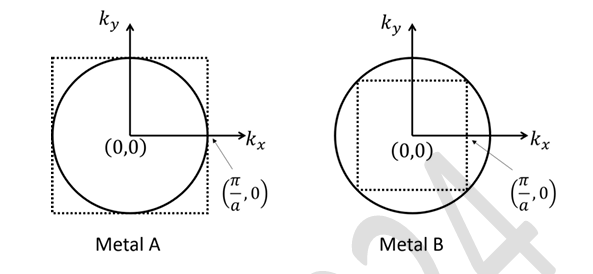
\includegraphics[width = 0.7\columnwidth]{fig/Q16.png}
    \caption*{}
    \label{fig:Q16}
\end{figure}
The electron concentrations in A and B are $n_A$ and $n_B$, respectively. The value of $\brak{\dfrac{n_B}{n_A}}$ is
\begin{enumerate}
    \item $3$
    \item $2$
    \item $3\sqrt{3}$
    \item $\sqrt{2}$
\end{enumerate}
\item Consider the induced nuclear fission reaction
\begin{align}
^{235}_{92}\mathrm{U} + n \rightarrow ^{93}_{37}\mathrm{Rb} + ^{141}_{55}\mathrm{Cs} + 2n
\end{align}
where neutron momenta in both initial and final states are negligible. The ratio of the kinetic energies (KE) of the daughter nuclei,
\begin{align}
\frac{\mathrm{KE} {(^{93}_{37}\mathrm{Rb})}}{\mathrm{KE}(^{141}_{55}\mathrm{Cs})} 
\end{align}
is \underline{\hspace{2cm}}
\begin{enumerate}
    \item $\dfrac{93}{141}$
    \item $\dfrac{141}{93}$
    \item $1$
    \item $0$
\end{enumerate}

\item The symbols C, D, $V_\text{in}$ and $V_0$ shown in the figure denote capacitor, ideal diode, input voltage and output voltage, respectively.
\begin{figure}[H]
    \centering
    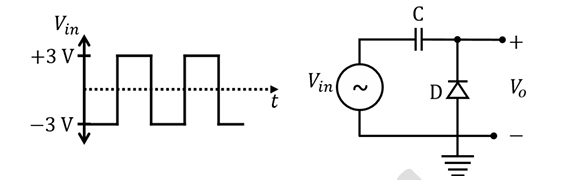
\includegraphics[width = 0.7\columnwidth]{fig/Q18(1).png}
    \caption*{}
    \label{fig:Q18(1)}
\end{figure}
Which one of the following output waveforms ($V_0$) is correct for the given input waveform ($V_\text{in}$)?
\begin{figure}[H]
    \centering
    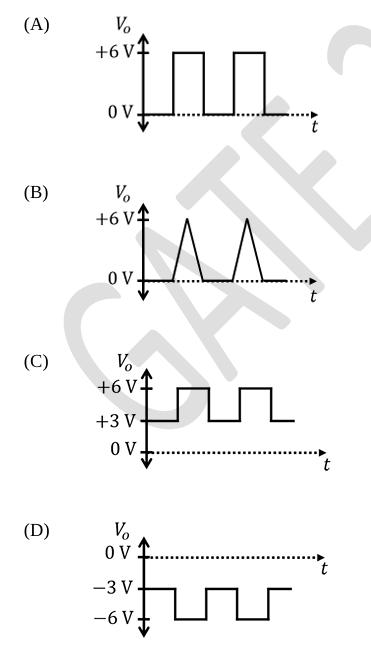
\includegraphics[width = 0.6\columnwidth]{fig/Q18(2).png}
    \caption*{}
    \label{fig: Q18(2)}
\end{figure}
\newpage
\item Let $N_e$ and $T_e$, respectively, denote number and kinetic energy of electrons produced in a nuclear beta decay. Which one of the following distributions is correct?
\begin{figure}[H]
    \centering
    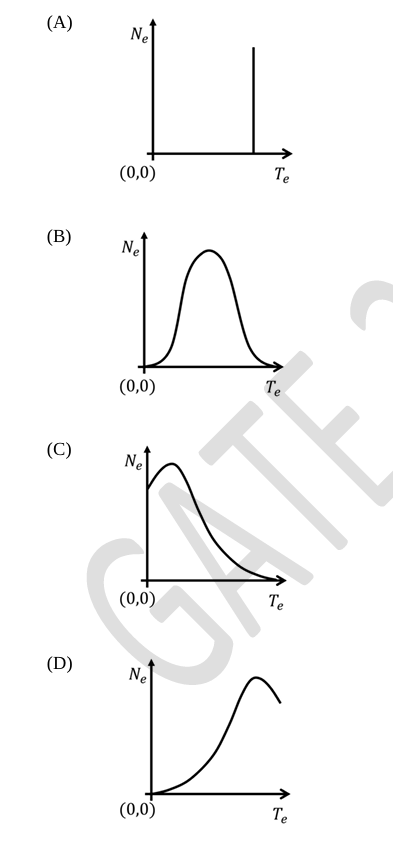
\includegraphics[width = 0.4\columnwidth]{fig/Q19.png}
    \caption*{}
    \label{fig: Q19}
\end{figure}
\item An infinitely long cylinder of radius $R$ carries a frozen-in magnetization $\vec{M} = k e^{-s} \hat{z}$, where $k$ is a constant and $s$ is the distance from the axis of cylinder. The magnetic permeability of free space is $\mu_0$. There is no free current present anywhere. The magnetic flux density ($\vec{B}$) inside the cylinder is
\begin{enumerate}
    \item $0$
    \item $\mu_0 k e^{-R} \hat{z}$
    \item $\mu_0 k e^{-s} \hat{z}$
    \item $\mu_0 k e^{-s} \brak{\dfrac{R}{s} } \hat{z}$
\end{enumerate}

\item Atomic numbers of V, Cr, Fe and Zn are 23, 24, 26 and 30, respectively. Which one of the following materials does NOT show an electron spin resonance (ESR) spectra?
\begin{enumerate}
    \item V
    \item Cr
    \item Fe
    \item Zn
\end{enumerate}

\item A particle is subjected to a potential
\begin{align}
V(x) =
\begin{cases}
\infty,  x \leq 0 \\
V_0,  a \leq x \leq b \\
0,  \text{elsewhere}
\end{cases}
\end{align}
Here, $a>0$ and $b>a$. If the energy of the particle $E < V_0$, which one of the following schematics is a valid quantum mechanical wavefunction ($\Psi$) for the system?
\begin{figure}[H]
    \centering
    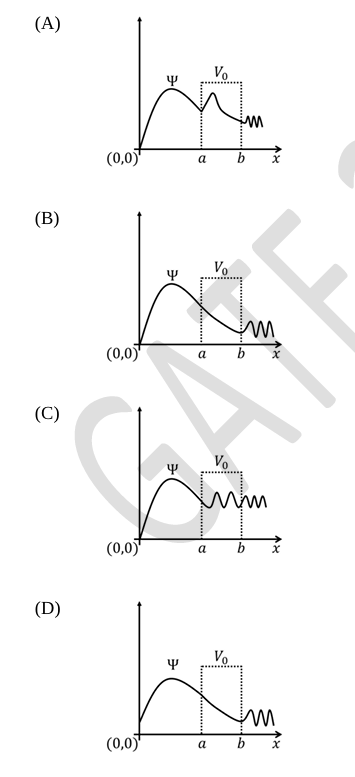
\includegraphics[width = 0.4\columnwidth]{fig/Q22.png}
    \caption*{}
    \label{fig: Q22}
\end{figure}
\item Let $\rho(\vec{p}, \vec{q}, t)$ be the phase space density of an ensemble of a system. The Hamiltonian of the system is $H(\vec{p}, \vec{q})$. If $\{A,B\}$ denotes the Poisson bracket of $A$ and $B$, then
\begin{align}
\frac{d\rho}{dt} = 0
\end{align}
implies
\begin{enumerate}
    \item $ \dfrac{\partial\rho}{\partial t} = 0$
    \item $ \dfrac{\partial\rho}{\partial t} \propto \{\rho, H\}$
    \item $\dfrac{\partial\rho}{\partial t} \propto \{ \rho, \frac{\vec{p} \cdot \vec{q}}{2}\}$
    \item $\dfrac{\partial\rho}{\partial t} \propto \{ \rho, \frac{\vec{q} \cdot \vec{q}}{2}\}$
    
\end{enumerate}

\item Consider the following circuit:
\begin{figure}[H]
    \centering
    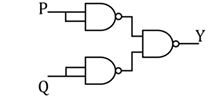
\includegraphics[width = 0.4\columnwidth]{fig/Q24(1).png}
    \caption*{}
    \label{fig: Q24}
\end{figure}
Suppose the input signal $P$ is
\begin{figure}[H]
    \centering
    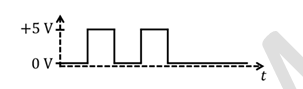
\includegraphics[width = 0.4\columnwidth]{fig/Q24(2).png}
    \caption*{}
    \label{fig: Q24}
\end{figure}
and the input signal $Q$ is
\begin{figure}[H]
    \centering
    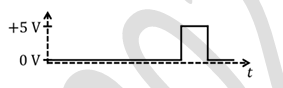
\includegraphics[width = 0.4\columnwidth]{fig/Q24(3).png}
    \caption*{}
    \label{fig: Q24}
\end{figure}
Which one of the following output signals is correct?
\begin{figure}[H]
    \centering
    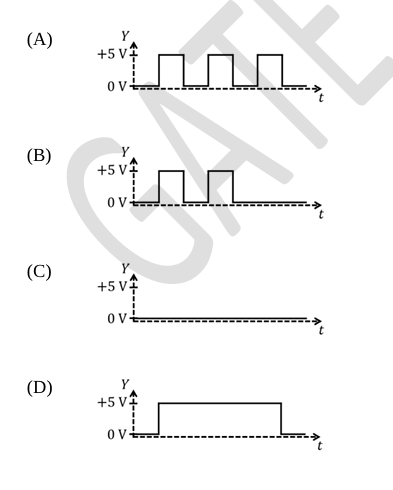
\includegraphics[width = 0.5\columnwidth]{fig/Q24(4).png}
    \caption*{}
    \label{fig: Q24}
\end{figure}
\item An inertial observer sees two spacecrafts S and T flying away from each other along $x$-axis with individual speed $0.5c$, where $c$ is the speed of light. The speed of T with respect to S is
\begin{enumerate}
    \item $\dfrac{4}{5} c$
    \item $\dfrac{4}{3} c$
    \item $c$
    \item $\dfrac{2}{3} c$
\end{enumerate}


\item Let P, R and R be three different nuclei. Which one of the following nuclear processes is possible?
\begin{enumerate}
    \item $\nu_e + ^{A}_{Z}P \rightarrow ^{A}_{Z+1}Q + e^{-}$
    \item $\nu_e + ^{A}_{Z}P \rightarrow ^{A}_{Z-1}R + e^{+}$
    \item $\nu_e + ^{A}_{Z}P \rightarrow ^{A}_{Z}P + e^{+} + e^{-}$
    \item $\nu_e + ^{A}_{Z}P \rightarrow ^{A}_{Z}P + \gamma$
\end{enumerate}

\item The temperature dependence of the electrical conductivity ($\sigma$) of three intrinsic semiconductors A, B and C is shown in figure.
\begin{figure}[H]
    \centering
    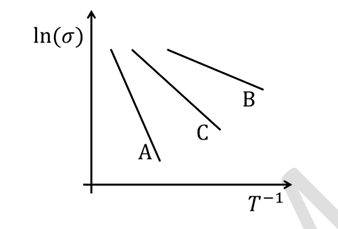
\includegraphics[width = 0.5\columnwidth]{fig/Q27.png}
    \caption*{}
    \label{fig: Q27}
\end{figure}
Let $E_A$, $E_B$ and $E_C$ be the bandgaps of A, B and C, respectively. Which one of the following relations is correct?
\begin{enumerate}
    \item $E_C > E_A > E_B$
    \item $E_B > E_C > E_A$
    \item $E_A > E_B > E_C$
    \item $E_A > E_C > E_B$
\end{enumerate}

\item Following trial wavefunctions
\begin{align*}
\phi_1 = e^{-Z'(r_1 + r_2)}
\end{align*}
and
\begin{align*}
    \phi_2 = e^{-Z'(r_1 + r_2)}(1 + g|\vec{r}_1 - \vec{r}_2|)
\end{align*}
are used to get a variational estimate of the ground state energy of the helium atom. $Z'$ and $g$ are the variational parameters, $\vec{r}_1$ and $\vec{r}_2$ are the position vectors of the electrons. Let $E_0$ be the exact ground state energy of the helium atom. $E_1$ and $E_2$ are the variational estimates of the ground state energy of the helium atom corresponding to $\phi_1$ and $\phi_2$, respectively. Which one of the following options is true?
\begin{enumerate}
    \item $E_1 \leq E_0, E_2 \leq E_0, E_1 \geq E_2$
    \item $E_1 \geq E_0, E_2 \leq E_0, E_1 \geq E_2$
    \item $E_1 \leq E_0, E_2 \geq E_0, E_1 \leq E_2$
    \item $E_1 \geq E_0, E_2 \geq E_0, E_1 \geq E_2$
\end{enumerate}
\item The wavefunction for a particle is given by the form $e^{-(i \alpha x + \beta)}$, where $\alpha$ and $\beta$ are real constants. In which one of the following potentials $V(x)$, the particle is moving?
\begin{enumerate}
    \item $V(x) \propto \alpha^2 x^2$
    \item $V(x) \propto e^{-\alpha x}$
    \item $V(x) = 0$
    \item $V(x) \propto \sin(\alpha x)$
\end{enumerate}

\item Consider a volume integral
\begin{align*}
    I = \int_V \nabla^2\brak{\frac{1}{r}} dV
\end{align*}
over a volume $V$, where $r = \sqrt{x^2 + y^2 + z^2}$. Which of the following statement is/are correct?
\begin{enumerate}
    \item $I = -4\pi$, if $r = 0$ is inside the volume $V$
    \item Integrand vanishes for $r \neq 0$
    \item $I = 0$, if $r = 0$ is not inside the volume $V$
    \item Integrand diverges as $r \rightarrow \infty$
\end{enumerate}
\item The complex function
\begin{align*}
e^{-\brak{\frac{2}{z-1}}}
\end{align*}
has \underline{\hspace{2cm}}
\begin{enumerate}
    \item a simple pole at $z=1$
    \item an essential singularity at $z=1$
    \item a residue equal to $-2$ at $z=1$
    \item a branch point at $z=1$
\end{enumerate}
\item
The minimum number of basic logic gates required to realize the Boolean expression $B \cdot (A + B) + A \cdot (\overline{B} + A)$ is \underline{\hspace{2cm}} \textit{(in integer)}.
\item
The vapor pressure ($P$) of solid ammonia is given by $\ln(P) = 23.03 - \frac{3754}{T}$, while that of liquid ammonia is given by $\ln(P) = 19.49 - \frac{3063}{T}$, where $T$ is the temperature in K. \\
The temperature of the triple point of ammonia is \underline{\hspace{2cm}} K (\textit{rounded off to two decimal places}).

\item
The electric field in a region depends only on $x$ and $y$ coordinates as
\begin{align*}
    \vec{E} = k \frac{(x\, \hat{x} + y\, \hat{y})}{x^2 + y^2}
\end{align*}
where $k$ is a constant. The flux of $\vec{E}$ through the surface of a sphere of radius $R$ with its center at the origin is $n\pi k R$, where the value of $n$ is \underline{\hspace{2cm}} (\textit{in integer}).

\item
The Hamiltonian of a system of $N$ particles in volume $V$ at temperature $T$ is
\begin{align*}
    H = \sum_{i=1}^{2N} a_i q_i^2 + \sum_{i=1}^{2N} b_i p_i^2
\end{align*}
where $a_i$ and $b_i$ are positive constants. The ensemble average of the Hamiltonian is $\alpha N k_B T$, where $k_B$ is the Boltzmann constant. The value of $\alpha$ is \underline{\hspace{2cm}} (\textit{in integer}).
\item Binding energy and rest mass energy of a two-nucleon bound state are denoted by $B$ and $mc^2$, respectively, where $c$ is the speed of light. The minimum energy of a photon required to dissociate the bound state is
\begin{enumerate}
    \item $B$
    \item $B \brak{ 1 + \dfrac{B}{2mc^2}} $
    \item $B \brak{ 1 - \dfrac{B}{2mc^2}} $
    \item $B - mc^2$
\end{enumerate}

\item The spin-orbit interaction in a hydrogen-like atom is given by the Hamiltonian
\begin{align*}
H' = -k\vec{L}\cdot \vec{S}
\end{align*}
where $k$ is a real constant. The splitting between levels $2p_{3/2}$ and $2p_{1/2}$ due to this interaction is
\begin{enumerate}
    \item $\dfrac{1}{2}kh^2$
    \item $\dfrac{3}{2}kh^2$
    \item $\dfrac{3}{4}kh^2$
    \item $2kh^2$
\end{enumerate}

\item
Consider the Lagrangian $L = m\dot{x}\dot{y} - m\omega_0^2 x y$. If $p_x$ and $p_y$ denote the generalized momenta conjugate to $x$ and $y$, respectively, then the canonical equations of motion are
\begin{enumerate}
    \item $\dot{x} = \dfrac{p_x}{m},\dot{p}_x = -m\omega_0^2 x, \dot{y} = \dfrac{p_y}{m}, \dot{p}_y = -m\omega_0^2 y$
    \item $\dot{x} = \dfrac{p_x}{m},\dot{p}_x = m\omega_0^2 y,\dot{y} = \dfrac{p_y}{m},\quad \dot{p}_y = m\omega_0^2 x$
    \item $\dot{x} = \dfrac{p_y}{m}, \dot{p}_x = -m\omega_0^2 y, \dot{y} = \dfrac{p_x}{m},\dot{p}_y = -m\omega_0^2 x$
    \item $\dot{x} = \dfrac{p_y}{m},\dot{p}_x = m\omega_0^2 y,\dot{y} = \dfrac{p_x}{m},\dot{p}_y = m\omega_0^2 x$
\end{enumerate}

\item The X-ray diffraction pattern of a monatomic cubic crystal with rigid spherical atoms of radius $1.56A$ shows several Bragg reflections of which the reflection appearing at the lowest $2\theta$ value is from (111) plane. If the wavelength of X-ray used is $0.78A$, the Bragg angle (in $2\theta$, \textit{rounded off to one decimal place}) corresponding to this reflection and the crystal structure, respectively, are
\begin{enumerate}
    \item 21.6$^\circ$ and body centered cubic
    \item 17.6$^\circ$ and face centered cubic
    \item 10.8$^\circ$ and body centered cubic
    \item 8.8$^\circ$ and face centered cubic
\end{enumerate}

\item In a parallel plate capacitor, the plate at $x=0$ is grounded and the plate at $x=d$ is maintained at a potential $V_0$. The space between the two plates is filled with a linear dielectric of permittivity $\epsilon = \epsilon_0\brak{1 + \frac{x}{d}}$, where $\epsilon_0$ is the permittivity of free space. Neglecting the edge effects, the electric field ($\vec{E}$) inside the capacitor is
\begin{enumerate}
    \item $-\dfrac{V_0}{(d + x)\ln 2}\,\hat{x}$
    \item $-\dfrac{V_0}{d}\,\hat{x}$
    \item $-\dfrac{V_0}{(d + x)}\,\hat{x}$
    \item $-\dfrac{V_0 d}{(d + x)x}\,\hat{x}$
\end{enumerate}

\item The equation of motion for the forced simple harmonic oscillator is
\begin{align*}
    \ddot{x}(t) + \omega^2 x(t) = F \cos(\omega t)
\end{align*}
where $x(0) = 0$ and $\dot{x}(0) = 0$. Which one of the following options is correct?
\begin{enumerate}
    \item $x(t) \propto t\sin(\omega t)$
    \item $x(t) \propto t\cos(\omega t)$
    \item $x(t) = \infty$
    \item $x(t) \propto e^{\omega t}$
\end{enumerate}
\item An atom is subjected to a weak uniform magnetic field $\vec{B}$. The number of lines in its Zeeman spectrum for transition from $n = 2, l = 1$ to $n = 1, l = 0$ is
\begin{enumerate}
    \item 8
    \item 10
    \item 12
    \item 5
\end{enumerate}

\item Consider two matrices: $P = \myvec {1 & 2 \\ 0 & 1} $ and $Q = \myvec{ 1 & 0 \\ 0 & 1 }$.\\
Which of the following statement is/are true?
\begin{enumerate}
    \item P and Q have same set of eigenvalues
    \item P and Q commute with each other
    \item P and Q have different sets of linearly independent eigenvectors
    \item P is diagonalizable
\end{enumerate}
\item An infinite one dimensional lattice extends along $x$-axis. At each lattice site there exists an ion with spin $\frac{1}{2}$. The spin can point either in $+z$ or $-z$ direction only. Let $S_P$, $S_F$, and $S_A$ denote the entropies of paramagnetic, ferromagnetic and antiferromagnetic configurations, respectively. Which of the following relation is/are true?
\begin{enumerate}
    \item $S_P > S_F$
    \item $S_A > S_F$
    \item $S_A = 4 S_F$
    \item $S_P > S_A$
\end{enumerate}

\item Consider a vector field $\vec{F} = (2xz + 3y^2)\hat{y} + 4yz^2 \hat{z}$. The closed path ($\Gamma$: A $\to$ B $\to$ C $\to$ D $\to$ A) in $z=0$ plane is shown in figure.
\begin{figure}[H]
    \centering
    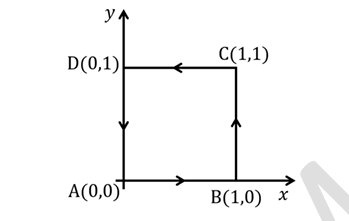
\includegraphics[width = 0.5\columnwidth]{fig/Q45.png}
    \caption*{}
    \label{fig: Q45}
\end{figure}
$\oint_\Gamma \vec{F}\cdot d\vec{l}$ denotes the line integral of $\vec{F}$ along the closed path $\Gamma$. Which of the following option is/are true?
\begin{enumerate}
    \item $ \oint_\Gamma \vec{F}\cdot d\vec{l} = 0$
    \item $\vec{F}$ is non-conservative
    \item $\nabla \cdot \vec{F} = 0$
    \item $\vec{F}$ can be written as the gradient of a scalar field
\end{enumerate}

\item Two point charges of charge $+q$ each are placed a distance $2d$ apart. A grounded solid conducting sphere of radius $a$ is placed midway between them. Assume $a^2 << d^2$. Which of the following statement is/are true?
\begin{enumerate}
    \item If $a > \dfrac{d}{8}$, the net force acting on the charges is directed towards each other
    \item The potential at the surface of the sphere is zero
    \item Total induced charge on the sphere is $\left( -\dfrac{2a q}{d} \right)$
    \item The potential at the center of the sphere is non-zero
\end{enumerate}

\item A particle of mass $m$ is moving in the potential
\begin{align*}
    V(x) =
\begin{cases}
V_0 + \dfrac{1}{2} m \omega_0^2 x^2,& x > 0\\
\infty,& x \leq 0
\end{cases}
\end{align*}

Figures P, Q, R and S show different combinations of the values of $\omega_0$ and $V_0$.
\begin{figure}[H]
    \centering
    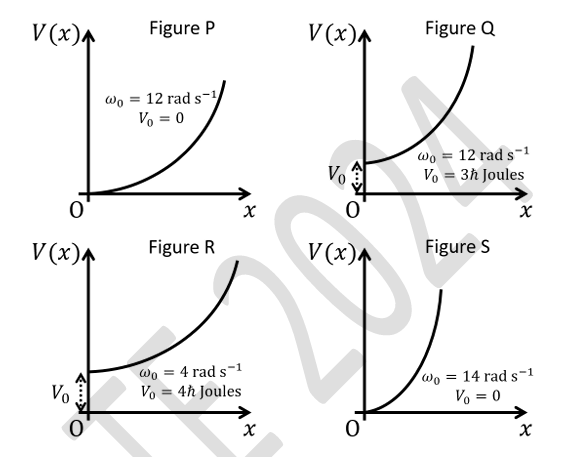
\includegraphics[width = 0.6\columnwidth]{fig/Q47.png}
    \caption*{}
    \label{fig: Q47}
\end{figure}
$E_j^{({P})}$, $E_j^{({Q})}$, $E_j^{({R})}$ and $E_j^{({S})}$ with $j=0,1,2,...$ are the eigen-energies of the $j$-th level for the potentials shown in figures P, Q, R and S, respectively. Which of the statement is/are true?
\begin{enumerate}
    \item $E_0^{({P})} = E_0^{({Q})}$
    \item $E_0^{({Q})} = E_0^{({S})}$
    \item $E_0^{({P})} = E_1^{({R})}$
    \item $E_0^{({R})} \neq E_0^{({Q})}$
\end{enumerate}

\item The non-relativistic Hamiltonian for a single electron atom is
\begin{align*}
    H_0 = \frac{p^2}{2m} - V(r)
\end{align*}

where $V(r)$ is the Coulomb potential and $m$ is the mass of the electron. Considering the spin-orbit interaction term
\begin{align*}
    H' = \frac{1}{2m^2c^2} \frac{1}{r} \frac{dV}{dr} \vec{L} \cdot \vec{S}
\end{align*}
added to $H_0$, which of the following statement is/are true?
\begin{enumerate}
    \item $H'$ commutes with $L^2$
    \item $H'$ commutes with $L_z$ and $S_z$
    \item For a given value of principal quantum number $n$ and orbital angular momentum quantum number $l$, there are $2(2l+1)$ degenerate eigenstates of $H_0$
    \item $H_0$, $L^2$, $S^2$, $L_z$ and $S_z$ have a set of simultaneous eigenstates
\end{enumerate}
\item Decays of mesons and baryons can be categorized as weak, strong and electromagnetic decays depending upon the interactions involved in the processes. Which of the following option is/are true?
\begin{enumerate}
    \item $\pi^0 \rightarrow \gamma \gamma$ is a weak decay
    \item $\Lambda^0 \rightarrow \pi^0 + p$ is an electromagnetic decay
    \item $K^0 \rightarrow \pi^+ + \pi^-$ is a weak decay
    \item $\Delta^{++} \rightarrow p + \pi^+$ is a strong decay
\end{enumerate}

\item An extrinsic semiconductor shown in figure carries a current of 2 mA along its length parallel to $+x$ axis.
\begin{figure}[H]   
\centering   
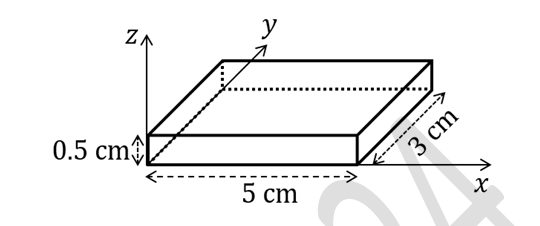
\includegraphics[width = 0.6\columnwidth]{fig/Q50.png}     \caption*{}  
\label{fig: Q50}
\end{figure}
When the majority charge carrier concentration is $12.5 \times 10^{13}$ cm$^{-3}$ and the sample is exposed to a constant magnetic field applied along the $+z$ direction, a Hall voltage of $20$ mV is measured with the negative polarity at $y=0$ plane. Take the electric charge as $1.6 \times 10^{-19}$ C. The concentration of minority charge carrier is negligible. Which of the following statement is/are true?
\begin{enumerate}
    \item The majority charge carrier is electron
    \item The magnitude of the applied magnetic field is $1$ Tesla
    \item The electric field corresponding to the Hall voltage is in the $+y$ direction
    \item The magnitude of Hall coefficient is $50,000$ m$^3$C$^{-1}$
\end{enumerate}

\item $A^{\alpha}$ and $B_{\beta}$ ($\alpha, \beta = 1,2,3, \dots, n$) are contravariant and covariant vectors, respectively. By convention, any repeated indices are summed over. Which of the following expression is/are tensors?
\begin{enumerate}
    \item $A^{\alpha} B_{\beta}$
    \item $\dfrac{A^{\alpha} B_{\beta}}{A^{\alpha} B_{\alpha}}$
    \item $\dfrac{A^{\alpha}}{B_{\beta}}$
    \item $A^{\alpha} + B_{\beta}$
\end{enumerate}

\item The temperature $T$ dependence of magnetic susceptibility $\chi$ (Column I) of certain magnetic materials (Column II) are given below. Which of the following option is/are correct?
\begin{figure}[H]  
\centering 
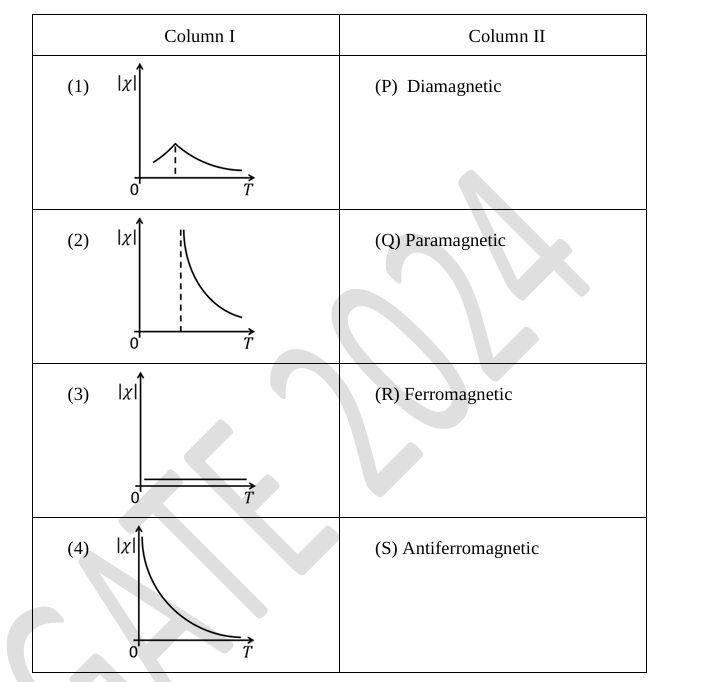
\includegraphics[width = 0.7\columnwidth]{fig/Q52.png}     \caption*{}  
\label{fig: Q52} 
\end{figure} 
\begin{enumerate}
    \item 2 -- P, 4 -- Q, 3 -- S
    \item 4 -- P, 1 -- Q, 2 -- R
    \item 4 -- Q, 2 -- R, 1 -- S
    \item 3 -- P, 4 -- Q, 2 -- R
\end{enumerate}

\item The curves P and Q schematically show the variation of X-ray intensity with wavelength at two different accelerating voltages for a given target material. In the figure $\lambda_1 = 0.25$ $A$, $\lambda_2 = 0.5$ $A$, $\lambda_3 = 1.0$ $A$, and $\lambda_4 = 2.25$ $A$. Take Plancks constant as $6.6 \times 10^{-34}$ Js, speed of light as $3 \times 10^{8}$ ms$^{-1}$ and elementary charge as $1.6 \times 10^{-19}$ C.
\begin{figure}[H]  
\centering  
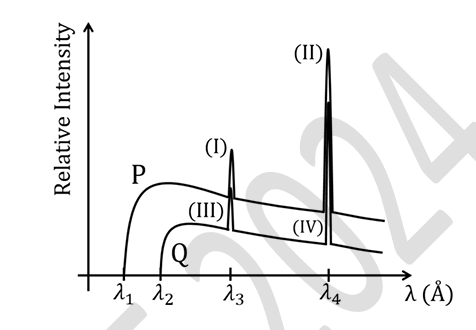
\includegraphics[width = 0.3\columnwidth]{fig/Q53.png}     \caption*{}  
\label{fig: Q53} 
\end{figure} 
Which of the following statement is/are true?
\begin{enumerate}
    \item The accelerating potential corresponding to curve P is greater than that of curve Q
    \item The accelerating potential applied to obtain curve Q is 24750 V
    \item Peaks (II) and (IV) correspond to radiative transitions from L to K shells
    \item Peaks (I) and (III) correspond to radiative transitions from N to K shells
\end{enumerate}

\item Apart from the acoustic modes, 9 optical modes are identified from the measurements of phonon dispersions of a solid with chemical formula $A_nB_m$, where $A$ and $B$ denote the atomic species, and $n$ and $m$ are integers. Which of the following combination of $n$ and $m$ is/are possible?
\begin{enumerate}
    \item n = 1, m = 1
    \item n = 2, m = 2
    \item n = 3, m = 1
    \item n = 4,m = 4
\end{enumerate}

\item An oscillating electric dipole of moment $\vec{d}(t) = d_0 \cos(\omega t)\,\hat{z}$ is placed at origin as shown in figure.
\begin{figure}[H]   
\centering    
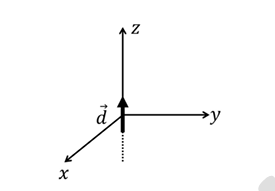
\includegraphics[width = .3\columnwidth]{fig/Q55.png}     \caption*{}  
\label{fig: Q55}
\end{figure} 
Consider a point $P(r, \theta, \phi)$ at a very large distance from the dipole. Here $r$, $\theta$ and $\phi$ are spherical polar coordinates. Which of the following statement is/are true for intensity of radiation?
\begin{enumerate}
    \item Intensity is zero if P is on the $z$ axis
    \item Intensity is zero at P$\brak{r = R, \theta = \frac{\pi}{2}, \phi = \frac{\pi}{4}}$
    \item Intensity at $Pr = R, \theta = \frac{\pi}{2}, \phi = \frac{\pi}{4}$ is greater than that at $P\brak{r = R,\, \theta = \frac{\pi}{4}, \phi = \frac{\pi}{4}}$
    \item Intensity at $P\brak{r = R, \theta = \frac{\pi}{2}, \phi = \frac{\pi}{4}}$ is equal to that at $P\brak{r = R, \theta = \frac{\pi}{4}, \phi = \frac{\pi}{4}}$
\end{enumerate}

\item The Fourier transform and its inverse transform are respectively defined as
$
\tilde{f}(\omega) = \frac{1}{\sqrt{2\pi}} \int_{-\infty}^{+\infty} f(x) e^{i\omega x} dx
$
and
$
f(x) = \frac{1}{\sqrt{2\pi}} \int_{-\infty}^{+\infty} \tilde{f}(\omega) e^{-i\omega x} d\omega.
$
Consider two functions $f$ and $g$. Another function $f * g$ is defined as
\begin{align*}
(f * g)(x) = \frac{1}{\sqrt{2\pi}} \int_{-\infty}^{+\infty} f(y) g(x - y) dy
\end{align*}
Which of the following relation is/are true?
Note: Tilde ($\sim$) denotes the Fourier transform.
\begin{enumerate}
    \item $f * g = g * f$
    \item $\widetilde{f * g} = \widetilde{g * f}$
    \item $\widetilde{f * g} = \widetilde{fg}$
    \item $\widetilde{f * g} = \tilde{f} \tilde{g}$
\end{enumerate}

\item A material behaves as a superconductor below a critical temperature $T_c$ and as a normal conductor above $T_c$. A magnetic field $\vec{B} = B\hat{z}$ is applied when $T > T_c$. The material is then cooled below $T_c$ in the presence of $\vec{B}$. Which of the following figure represent the correct configuration of magnetic field lines?
\begin{figure}[H]    
\centering    
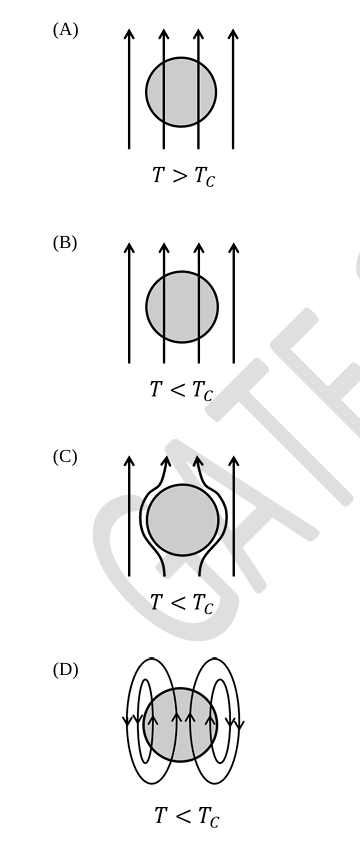
\includegraphics[width = 0.3\columnwidth]{fig/Q57.png}     \caption*{}   
\label{fig: Q57} 
\end{figure}
\item A typical biasing of a silicon transistor is shown in figure.
\begin{figure}[H]
\centering    
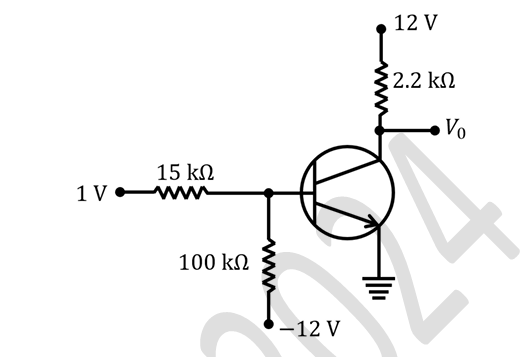
\includegraphics[width = 0.3\columnwidth]{fig/Q58.png}     \caption*{}  
\label{fig: Q58}
\end{figure} 
The value of common-emitter current gain $\beta$ for the transistor is 100. Ignore reverse saturation current. The output voltage $V_0$ (in V) is \underline{\hspace{2cm}} \textit{(in integer)}.

\item The canonical partition function of an ideal gas is
\begin{align*}
    Q(T, V, N) = \frac{1}{N!} \sbrak{ \frac{V}{{\lambda(T)}^3} ^N}
\end{align*}
where $T, V, N$ and $\lambda(T)$ denote temperature, volume, number of particles, and thermal de Broglie wavelength, respectively. Let $k_B$ be the Boltzmann constant and $\mu$ be the chemical potential. Take $\ln(N!) = N \ln(N) - N$.
If the number density $ \brak{\frac{N}{V}} $ is $2.5 \times 10^{25} {m}^{-3}$ at a temperature $T$, then
$
\frac{e^{\mu / (k_B T)}}{ \lambda(T) ^3} \times 10^{-25}
$
is \underline{\hspace{2cm}} $\mathrm{m}^{-3}$ \textit{(rounded off to one decimal place)}.

\item Lagrangian of a particle of mass $m$ is $L = \frac{1}{2} m \dot{x}^2 - \lambda x^4$, where $\lambda$ is a positive constant. If the particle oscillates with total energy $E$, then the time period of oscillations is
\begin{align*}
    a \int_0^{\brak{{\frac{E}{\lambda}}^{1/4}}} \frac{dx}{\sqrt{(\frac{2}{m})(E-\lambda x^4)}}
\end{align*}


The value of $a$ is \underline{\hspace{2cm}} \textit{(in integer)}.

\item A particle of mass $m$ in an infinite potential well of width $a$ is subjected to a perturbation, $V = \frac{h^2}{4 m a^2}$ as shown in figure, where $h$ is Plancks constant.
\begin{figure}[H]   
\centering    
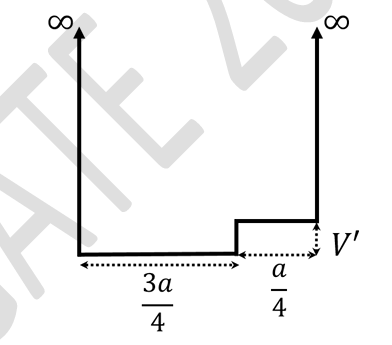
\includegraphics[width = 0.4\columnwidth]{fig/Q61.png}     \caption*{}  
\label{fig: 61} 
\end{figure} 
The first order energy shift of the fourth energy eigenstate due to this perturbation is
\begin{align*}
\frac{h^2}{N m a^2}
\end{align*}
The value of $N$ is \underline{\hspace{2cm}} \textit{(in integer)}.

\item Consider a three-dimensional system of non-interacting bosons with zero chemical potential. The energy of the system $\epsilon \propto k^2$, where $k$ is the wavevector. The low temperature specific heat of the system at constant volume depends on the temperature as $C_V \propto T^{\dfrac{n}{2}}$. The value of $n$ is \underline{\hspace{2cm}} \textit{(in integer)}.

\item Consider the operational amplifier circuit shown in figure.
\begin{figure}[H]  
\centering   
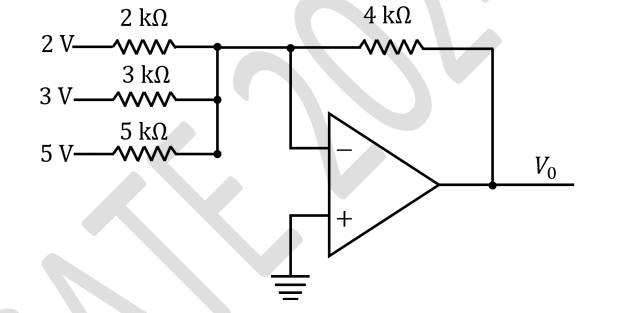
\includegraphics[width = 0.6\columnwidth]{fig/Q63.png}     \caption*{}  
\label{fig: Q63}
\end{figure} 
The output voltage $V_0$ is \underline{\hspace{2cm}} V \textit{(in integer)}.

\item An electron in the Coulomb field of a proton is in the following state of coherent superposition of orthonormal states $\psi_{nlm}$
\begin{align*}
\Psi = \frac{1}{3}\psi_{100} + \frac{1}{\sqrt{3}}\psi_{210} - \frac{\sqrt{5}}{3}\psi_{320}
\end{align*}
Let $E_1, E_2, E_3$ represent the first three energy levels of the system. A sequence of measurements is done on the same system at different times. Energy is measured first at time $t_1$ and the outcome is $E_2$. Then total angular momentum is measured at time $t_2 > t_1$ and finally energy is measured again at $t_3 > t_2$. The probability of finding the system in a state with energy $E_2$ after the final measurement is $P/9$. The value of $P$ is \underline{\hspace{2cm}} \textit{(in integer)}.

\item According to the nuclear shell model, the absolute value of the difference in magnetic moments of $^{15}*{8}\mathrm{O}$ and $^{15}*{7}\mathrm{N}$, in the units of nuclear magneton ($\mu_N$) is $a/3$.
The magnitude of $a$ is \underline{\hspace{2cm}} \textit{(in integer)}.
\end{enumerate}

\end{document}